% Created by tikzDevice version 0.12.6 on 2026-05-14 21:28:40
% !TEX encoding = UTF-8 Unicode
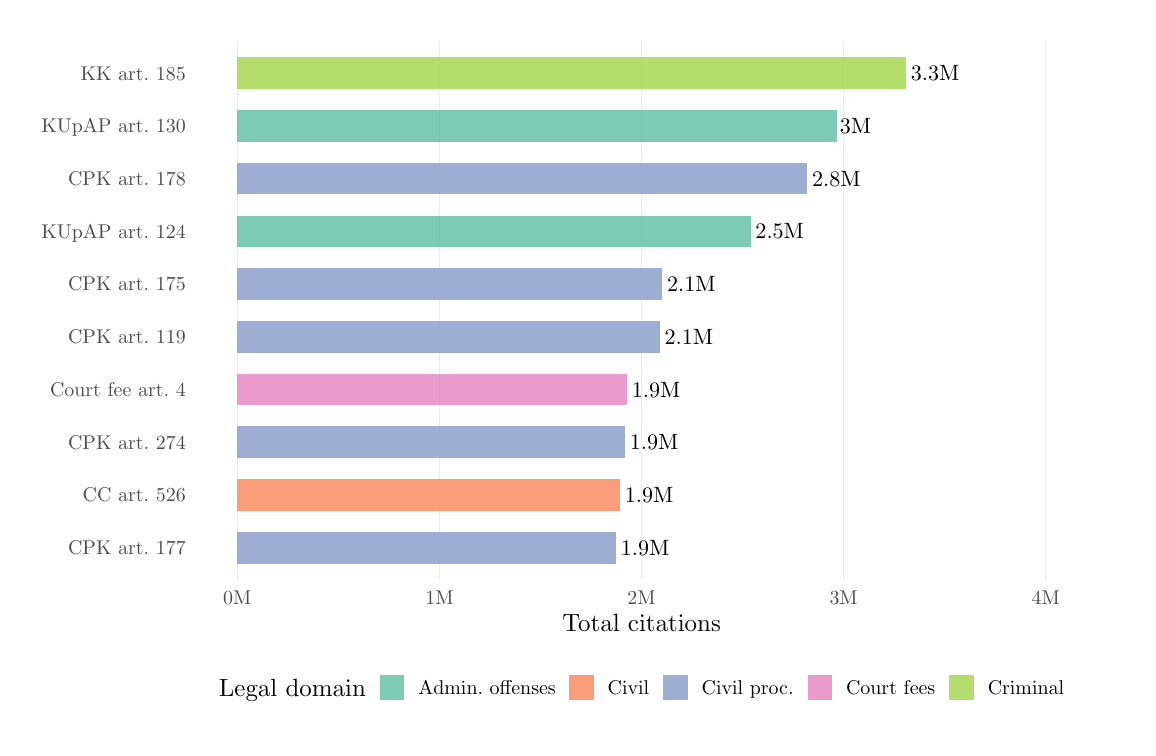
\begin{tikzpicture}[x=1pt,y=1pt]
\definecolor{fillColor}{RGB}{255,255,255}
\path[use as bounding box,fill=fillColor,fill opacity=0.00] (0,0) rectangle (397.48,252.94);
\begin{scope}
\path[clip] (  0.00,  0.00) rectangle (397.48,252.94);
\definecolor{fillColor}{RGB}{255,255,255}

\path[fill=fillColor] ( -0.00,  0.00) rectangle (397.48,252.95);
\end{scope}
\begin{scope}
\path[clip] ( 61.16, 53.56) rectangle (382.48,247.95);
\definecolor{drawColor}{gray}{0.92}

\path[draw=drawColor,line width= 0.5pt,line join=round] ( 75.76, 53.56) --
	( 75.76,247.95);

\path[draw=drawColor,line width= 0.5pt,line join=round] (148.79, 53.56) --
	(148.79,247.95);

\path[draw=drawColor,line width= 0.5pt,line join=round] (221.82, 53.56) --
	(221.82,247.95);

\path[draw=drawColor,line width= 0.5pt,line join=round] (294.85, 53.56) --
	(294.85,247.95);

\path[draw=drawColor,line width= 0.5pt,line join=round] (367.88, 53.56) --
	(367.88,247.95);
\definecolor{fillColor}{RGB}{166,216,84}

\path[fill=fillColor,fill opacity=0.85] ( 75.76,230.79) rectangle (317.41,242.23);
\definecolor{fillColor}{RGB}{102,194,165}

\path[fill=fillColor,fill opacity=0.85] ( 75.76,211.74) rectangle (292.35,223.17);
\definecolor{fillColor}{RGB}{141,160,203}

\path[fill=fillColor,fill opacity=0.85] ( 75.76,192.68) rectangle (281.72,204.11);
\definecolor{fillColor}{RGB}{102,194,165}

\path[fill=fillColor,fill opacity=0.85] ( 75.76,173.62) rectangle (261.23,185.06);
\definecolor{fillColor}{RGB}{141,160,203}

\path[fill=fillColor,fill opacity=0.85] ( 75.76,154.57) rectangle (229.30,166.00);

\path[fill=fillColor,fill opacity=0.85] ( 75.76,135.51) rectangle (228.41,146.94);
\definecolor{fillColor}{RGB}{231,138,195}

\path[fill=fillColor,fill opacity=0.85] ( 75.76,116.45) rectangle (216.59,127.89);
\definecolor{fillColor}{RGB}{141,160,203}

\path[fill=fillColor,fill opacity=0.85] ( 75.76, 97.40) rectangle (215.86,108.83);
\definecolor{fillColor}{RGB}{252,141,98}

\path[fill=fillColor,fill opacity=0.85] ( 75.76, 78.34) rectangle (214.04, 89.77);
\definecolor{fillColor}{RGB}{141,160,203}

\path[fill=fillColor,fill opacity=0.85] ( 75.76, 59.28) rectangle (212.62, 70.72);
\definecolor{drawColor}{RGB}{0,0,0}

\node[text=drawColor,anchor=base west,inner sep=0pt, outer sep=0pt, scale=  0.80] at (319.15,233.77) {3.3M};

\node[text=drawColor,anchor=base west,inner sep=0pt, outer sep=0pt, scale=  0.80] at (293.48,214.71) {3M};

\node[text=drawColor,anchor=base west,inner sep=0pt, outer sep=0pt, scale=  0.80] at (283.47,195.65) {2.8M};

\node[text=drawColor,anchor=base west,inner sep=0pt, outer sep=0pt, scale=  0.80] at (262.98,176.60) {2.5M};

\node[text=drawColor,anchor=base west,inner sep=0pt, outer sep=0pt, scale=  0.80] at (231.05,157.54) {2.1M};

\node[text=drawColor,anchor=base west,inner sep=0pt, outer sep=0pt, scale=  0.80] at (230.16,138.48) {2.1M};

\node[text=drawColor,anchor=base west,inner sep=0pt, outer sep=0pt, scale=  0.80] at (218.34,119.43) {1.9M};

\node[text=drawColor,anchor=base west,inner sep=0pt, outer sep=0pt, scale=  0.80] at (217.61,100.37) {1.9M};

\node[text=drawColor,anchor=base west,inner sep=0pt, outer sep=0pt, scale=  0.80] at (215.79, 81.31) {1.9M};

\node[text=drawColor,anchor=base west,inner sep=0pt, outer sep=0pt, scale=  0.80] at (214.36, 62.26) {1.9M};
\end{scope}
\begin{scope}
\path[clip] (  0.00,  0.00) rectangle (397.48,252.94);
\definecolor{drawColor}{gray}{0.30}

\node[text=drawColor,anchor=base east,inner sep=0pt, outer sep=0pt, scale=  0.72] at ( 57.11, 62.52) {CPK art.\ 177};

\node[text=drawColor,anchor=base east,inner sep=0pt, outer sep=0pt, scale=  0.72] at ( 57.11, 81.58) {CC art.\ 526};

\node[text=drawColor,anchor=base east,inner sep=0pt, outer sep=0pt, scale=  0.72] at ( 57.11,100.63) {CPK art.\ 274};

\node[text=drawColor,anchor=base east,inner sep=0pt, outer sep=0pt, scale=  0.72] at ( 57.11,119.69) {Court fee art.\ 4};

\node[text=drawColor,anchor=base east,inner sep=0pt, outer sep=0pt, scale=  0.72] at ( 57.11,138.75) {CPK art.\ 119};

\node[text=drawColor,anchor=base east,inner sep=0pt, outer sep=0pt, scale=  0.72] at ( 57.11,157.80) {CPK art.\ 175};

\node[text=drawColor,anchor=base east,inner sep=0pt, outer sep=0pt, scale=  0.72] at ( 57.11,176.86) {KUpAP art.\ 124};

\node[text=drawColor,anchor=base east,inner sep=0pt, outer sep=0pt, scale=  0.72] at ( 57.11,195.92) {CPK art.\ 178};

\node[text=drawColor,anchor=base east,inner sep=0pt, outer sep=0pt, scale=  0.72] at ( 57.11,214.97) {KUpAP art.\ 130};

\node[text=drawColor,anchor=base east,inner sep=0pt, outer sep=0pt, scale=  0.72] at ( 57.11,234.03) {KK art.\ 185};
\end{scope}
\begin{scope}
\path[clip] (  0.00,  0.00) rectangle (397.48,252.94);
\definecolor{drawColor}{gray}{0.30}

\node[text=drawColor,anchor=base,inner sep=0pt, outer sep=0pt, scale=  0.72] at ( 75.76, 44.56) {0M};

\node[text=drawColor,anchor=base,inner sep=0pt, outer sep=0pt, scale=  0.72] at (148.79, 44.56) {1M};

\node[text=drawColor,anchor=base,inner sep=0pt, outer sep=0pt, scale=  0.72] at (221.82, 44.56) {2M};

\node[text=drawColor,anchor=base,inner sep=0pt, outer sep=0pt, scale=  0.72] at (294.85, 44.56) {3M};

\node[text=drawColor,anchor=base,inner sep=0pt, outer sep=0pt, scale=  0.72] at (367.88, 44.56) {4M};
\end{scope}
\begin{scope}
\path[clip] (  0.00,  0.00) rectangle (397.48,252.94);
\definecolor{drawColor}{RGB}{0,0,0}

\node[text=drawColor,anchor=base,inner sep=0pt, outer sep=0pt, scale=  0.90] at (221.82, 34.71) {Total citations};
\end{scope}
\begin{scope}
\path[clip] (  0.00,  0.00) rectangle (397.48,252.94);
\definecolor{drawColor}{RGB}{0,0,0}

\node[text=drawColor,anchor=base west,inner sep=0pt, outer sep=0pt, scale=  0.90] at ( 69.10, 11.38) {Legal domain};
\end{scope}
\begin{scope}
\path[clip] (  0.00,  0.00) rectangle (397.48,252.94);
\definecolor{fillColor}{RGB}{102,194,165}

\path[fill=fillColor,fill opacity=0.85] (127.29, 10.08) rectangle (136.09, 18.88);
\end{scope}
\begin{scope}
\path[clip] (  0.00,  0.00) rectangle (397.48,252.94);
\definecolor{fillColor}{RGB}{252,141,98}

\path[fill=fillColor,fill opacity=0.85] (195.72, 10.08) rectangle (204.51, 18.88);
\end{scope}
\begin{scope}
\path[clip] (  0.00,  0.00) rectangle (397.48,252.94);
\definecolor{fillColor}{RGB}{141,160,203}

\path[fill=fillColor,fill opacity=0.85] (229.67, 10.08) rectangle (238.47, 18.88);
\end{scope}
\begin{scope}
\path[clip] (  0.00,  0.00) rectangle (397.48,252.94);
\definecolor{fillColor}{RGB}{231,138,195}

\path[fill=fillColor,fill opacity=0.85] (281.84, 10.08) rectangle (290.64, 18.88);
\end{scope}
\begin{scope}
\path[clip] (  0.00,  0.00) rectangle (397.48,252.94);
\definecolor{fillColor}{RGB}{166,216,84}

\path[fill=fillColor,fill opacity=0.85] (333.05, 10.08) rectangle (341.85, 18.88);
\end{scope}
\begin{scope}
\path[clip] (  0.00,  0.00) rectangle (397.48,252.94);
\definecolor{drawColor}{RGB}{0,0,0}

\node[text=drawColor,anchor=base west,inner sep=0pt, outer sep=0pt, scale=  0.72] at (141.17, 12.00) {Admin.\ offenses};
\end{scope}
\begin{scope}
\path[clip] (  0.00,  0.00) rectangle (397.48,252.94);
\definecolor{drawColor}{RGB}{0,0,0}

\node[text=drawColor,anchor=base west,inner sep=0pt, outer sep=0pt, scale=  0.72] at (209.59, 12.00) {Civil};
\end{scope}
\begin{scope}
\path[clip] (  0.00,  0.00) rectangle (397.48,252.94);
\definecolor{drawColor}{RGB}{0,0,0}

\node[text=drawColor,anchor=base west,inner sep=0pt, outer sep=0pt, scale=  0.72] at (243.55, 12.00) {Civil proc.};
\end{scope}
\begin{scope}
\path[clip] (  0.00,  0.00) rectangle (397.48,252.94);
\definecolor{drawColor}{RGB}{0,0,0}

\node[text=drawColor,anchor=base west,inner sep=0pt, outer sep=0pt, scale=  0.72] at (295.72, 12.00) {Court fees};
\end{scope}
\begin{scope}
\path[clip] (  0.00,  0.00) rectangle (397.48,252.94);
\definecolor{drawColor}{RGB}{0,0,0}

\node[text=drawColor,anchor=base west,inner sep=0pt, outer sep=0pt, scale=  0.72] at (346.93, 12.00) {Criminal};
\end{scope}
\end{tikzpicture}
